\documentclass{article}%
\usepackage[T1]{fontenc}%
\usepackage[utf8]{inputenc}%
\usepackage{lmodern}%
\usepackage{textcomp}%
\usepackage{lastpage}%
\usepackage[head=40pt,margin=0.5in,bottom=0.6in]{geometry}%
\usepackage{graphicx}%
%
\title{\textbf{Denuncian que directiva del HUC amenaza con armas a empleados que protestan}}%
\author{El Nacional Web}%
\date{13/11/2018}%
%
\begin{document}%
\normalsize%
\maketitle%
\textbf{URL: }%
http://www.el{-}nacional.com/noticias/sociedad/denuncian{-}que{-}directiva{-}del{-}huc{-}amenaza{-}con{-}armas{-}empleados{-}que{-}protestan\_259541\newline%
%
\textbf{Periodico: }%
EN, %
ID: %
259541, %
Seccion: %
Sociedad\newline%
%
\textbf{Palabras Claves: }%
Hospitales, Sociedad\newline%
%
\textbf{Derecho: }%
1.3%
, Otros Derechos: %
2.1%
, Sub Derechos: %
1.3.3, 2.1.1%
\newline%
%
\textbf{EP: }%
SI\newline%
\newline%
%
\textbf{\textit{Aseguran que los empleados del centro de salud han renunciado por las condiciones del lugar. Parte del personal que llegó a denunciar las condiciones hoy se encuentra bajo tratamiento psiquiátrico por las amenazas y persecuciones de las que fueron víctimas}}%
\newline%
\newline%
%
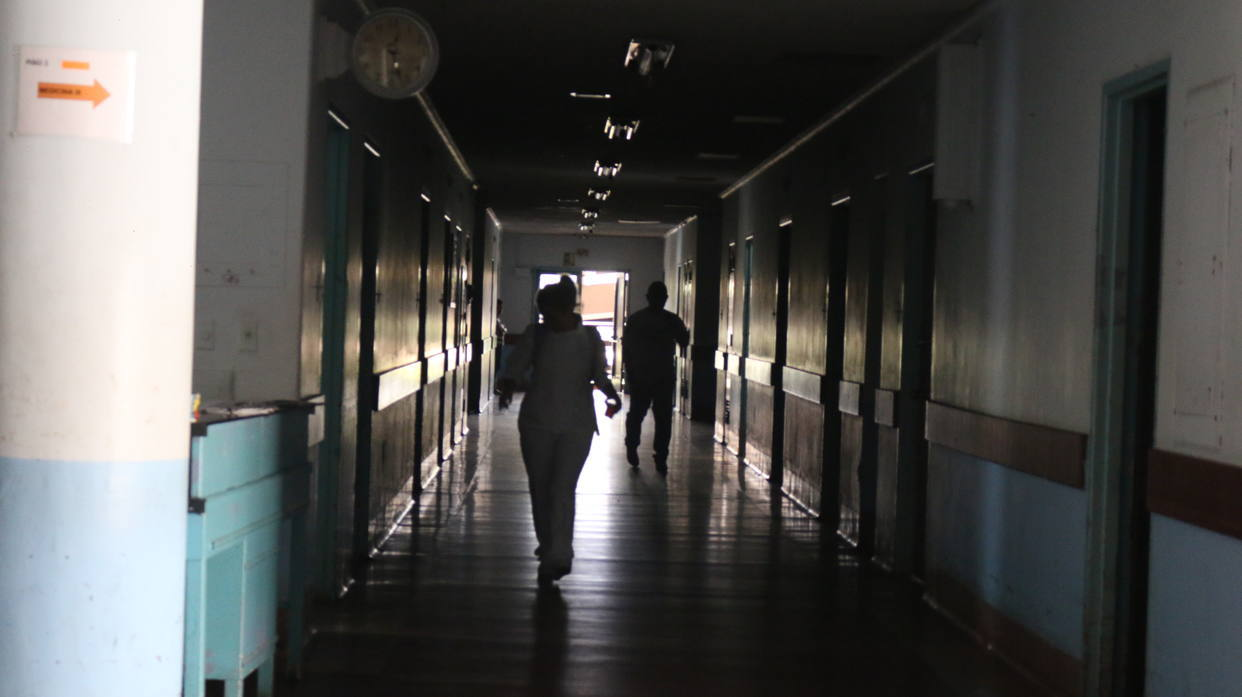
\includegraphics[width=300px]{135.jpg}%
\newline%
%
Una trabajadora del Hospital Universitario de Caracas (HUC) denunció que el director del centro de salud, Fernando Alvarado, amenaza con un grupo de personas a los pacientes y empleados que denuncian las condiciones del lugar.%
\newline%
%
“Desde que llegó el director Fernando Alvarado implementó los grupos de choque: los que amenazan, los que maltratan a los pacientes y a los trabajadores por reclamar”, aseguró a~El Nacional Web.%
\newline%
%
Explicó que uno de los sujetos encargado de las agresiones empujó y pateó a una mujer mayor de 50 años de edad. La situación fue denunciada ante la subdirectora; sin embargo, señala que tampoco recibieron una respuesta positiva de su parte.%
\newline%
%
“Regresamos y la subdirectora Anaida González volvió con lo mismo a amenazar a los trabajadores con pistola y demás”, aseveró.%
\newline%
%
La trabajadora dijo que tanto ella como sus compañeras sienten miedo por la situación, por lo que ciertas empleadas que alguna vez llegaron a protestar tuvieron que tomar un reposo psiquiátrico por las persecuciones y amenazas de muerte de las que eran víctimas.%
\newline%
%
“En estos momentos siento miedo, porque hablamos de una directiva, de una mujer que ya le ha sacado pistolas a las trabajadoras”, comentó~al tiempo que detalló que algunos trabajadores han renunciado tanto por la falta de~condiciones como por las amenazas.%
\newline%
%
Un solo ascensor%
\newline%
%
Agregó que solo cuentan con un ascensor para cubrir la demanda del HUC, situación que ha sido denunciada por las trabajadoras del departamento de Nutrición y Dietética en la dirección del hospital.%
\newline%
%
La empleada señaló que el único aparato que hay en el centro de salud es utilizado para movilizar comida, cadáveres y pacientes, lo que además de ir en contra de la higiene del lugar, complica la dinámica del hospital.%
\newline%
%
“Por ahí bajan a los muertos, suben a los pacientes, lo usan para todo. Entonces, ellos tenían que subir la comida y no pueden porque tienen que subir a los pacientes”, explicó.%
\newline%
%
Añadió que la alimentación de los pacientes es deficiente. “Lo único que se les está dando a los pacientes es bollito con caraota”, destacó.%
\newline%
%
\end{document}